\documentclass[conference]{IEEEtran}
% Shared look for the Rapport papers: packages and TikZ styles for the diagrams.
\usepackage[T1]{fontenc}
\usepackage{amsmath,amssymb}
\usepackage{graphicx}
\usepackage{booktabs}
\usepackage{tabularx}
\usepackage{array}
\usepackage{tikz}
\usetikzlibrary{arrows.meta,positioning,fit,backgrounds,calc,shapes.geometric,shapes.misc}
\usepackage{url}
\usepackage[hidelinks]{hyperref}
\graphicspath{{../figures/}}
\tikzset{
  >={Stealth[length=1.8mm]},
  box/.style={draw, rounded corners=2pt, align=center, font=\scriptsize, minimum height=7mm, inner sep=2pt, fill=#1},
  box/.default=cyan!8,
  code/.style={box=cyan!8},
  llm/.style={box=orange!12},
  io/.style={box=gray!10},
  unity/.style={box=green!10},
  bad/.style={box=red!8},
  good/.style={box=green!12},
  decision/.style={draw, diamond, aspect=2.2, align=center, font=\scriptsize, inner sep=1pt, fill=yellow!12},
  state/.style={draw, circle, align=center, font=\scriptsize, minimum size=12mm, fill=#1},
  state/.default=cyan!8,
  lab/.style={font=\tiny, align=center},
}
\newcolumntype{Y}{>{\raggedright\arraybackslash}X}


\begin{document}

\title{Rapport: An Embodied, On-Device Psychiatric Standardised Patient Driven by a Research-Grounded Digital Twin}

\author{\IEEEauthorblockN{Faaz Khan Mohammad}
\IEEEauthorblockA{Rapport project\\
Email: faazkhn1000@gmail.com}}

\maketitle

\begin{abstract}
Students learn psychiatric interviewing by practising with standardised patients: trained actors who play a patient in a timed exam station
(an OSCE). Actors are scarce, costly and hard to keep consistent, and today's AI patient simulators are mostly text chats that run in the cloud
and do not keep track of trust or mood. We present Rapport, a 3D patient that a student talks to out loud, running entirely on one laptop. The
patient's behaviour is set by a Digital Twin: a clear, inspectable model of the patient's story, memories that unlock with trust, feelings, mood and
choice of behaviour, built from ideas in published patient simulators. In the current version, ordinary code makes the decisions (what the
doctor's last sentence did, how trust changes, how guarded the patient is, which behaviours are allowed), and then one call to a local language
model puts the decision into words; every sentence is checked before it is spoken. The patient's posture, gaze and face follow the Twin's emotion.
Requests for a physical examination (``hold out your hands'') are recognised by rules (385 test sentences, 100\% correct, no false triggers), and
an examiner can watch the Twin's state live. Four draft stations (moderate depression, two ward scenarios and alcohol withdrawal) run on four patient
bodies, with patients that vary by seed and six conversation styles. On an Apple M5 Pro laptop the patient starts speaking a median 1.82\,s after the
student stops. In 14 held-out conversations, each run three times and marked by a different AI model and then by hand, the Twin had no jailbreak or
portrayal failures, disclosed suicidal thoughts every time they were unlocked and asked about kindly, and behaved more like a varied person than its
previous version, with equal accuracy. The debrief scores the student on what the patient actually showed and said. Ratings by psychiatry faculty
and a student pilot are still to come.
\end{abstract}

\begin{IEEEkeywords}
standardised patients, OSCE, psychiatry education, virtual patients, large language models, on-device AI
\end{IEEEkeywords}

\section{Introduction}
The psychiatric interview is learned by doing. A trainee has to notice slow speech and a lowered gaze, ask open questions, earn enough trust for a
patient to admit a wish not to wake up, and assess risk properly, all inside a timed OSCE station \cite{harden1975osce}. Standardised patient actors
make this possible, but they are costly, not always available, and hard to keep consistent between students \cite{piot2021simulation}.

AI patient simulators based on large language models have grown quickly. Psychiatric ones now model a patient's thinking patterns, resistance and
trust-gated disclosure \cite{wang2024patient,lee2025psyche,sabour2026patientact}. For OSCE practice, three gaps remain:
\begin{itemize}
\item \textbf{No body.} Most simulators are text chats, but psychiatric assessment depends on speech rate, pauses, facial expression and posture.
\item \textbf{Too slow to talk to.} Rich patient agents use several model calls per turn, which is too slow for spoken conversation on local hardware.
\item \textbf{A black box in the cloud.} Examiners cannot see why a simulated patient shared or held something back, and cloud models send student
audio off the premises.
\end{itemize}

\textbf{Contributions.}
C1: Rapport, an on-device, spoken 3D standardised patient for psychiatry and addiction OSCEs (four draft stations, four patient bodies, seeded patients
with six conversation styles).
C2: the Digital Twin, an explicit patient-mind model that combines ideas from published simulators and decides in code before a single model call.
C3: a fast-and-slow design that keeps one structured call on the critical path, with measured speed and a playback hold that keeps speech smooth
on a busy laptop.
C4: a live examiner view of the Twin.
C5: physical examination and body language driven by the Twin.
C6: a student assessment grounded in the literature.
C7: an evaluation suite and release gates for made-up facts, jailbreaks, portrayal and safety, with a learning loop that only accepts changes that pass.
Companion papers give the Twin's validation, the system architecture and the memory-matching method in more depth.

\section{Related Work}
\textbf{Psychiatric AI patients.} Chen et al.\ built chatbots validated by clinicians for depression interviews \cite{chen2023llmempowered};
PATIENT-$\Psi$ bases patients on expert cognitive models with six conversation styles \cite{wang2024patient}; PSYCHE builds a Mental Status Exam
framework to evaluate assessment agents \cite{lee2025psyche}; PatientAct adds trust-gated memory, reactions and resistance \cite{sabour2026patientact};
PatientHub collects many simulators \cite{sabour2026patienthub}; Roleplay-doh lets experts steer a patient with written principles
\cite{louie2024roleplaydoh}. \textbf{Patients that learn.} EvoPatient improves patients through simulated doctor--patient practice and a checked
library of past replies \cite{du2024llms}; MedAgentSim and Agent Hospital evolve agents in simulated clinics \cite{almansoori2025selfevolving,li2024agent}.
\textbf{Patients with bodies and voices.} Design guidelines for psychiatric virtual patients predate language models \cite{dupuy2020guidelines};
recent language-model 3D patients include Voigt et al.\ \cite{voigt2025llmpowered} and SOPHIE \cite{haut2025ai}; SimPatient and MedSimAI add feedback
on the student's performance \cite{steenstra2025scaffolding,hicke2025medsimai}. \textbf{Does it help?} A randomised trial found that patient simulation
with structured feedback improved students' clinical decisions \cite{brugge2024llm}; AI scoring of OSCE interview transcripts agrees with experts
within one point 67--87\% of the time \cite{geathers2025benchmarking}; a 2026 meta-analysis supports AI virtual patients for psychiatric interview training
\cite{kilincel2026meta}. AI judges are cheap but biased \cite{zheng2023judging}. \textbf{Digital brains.} The Brain/MINDS Digital Brain programme
\cite{brainminds} builds data-driven models of the brain; the Twin is not a brain model and only borrows its ideas as behaviour rules (for example, trust
changes when expectations are not met).

\section{What a Student Experiences}

\begin{figure}[t]
\centering
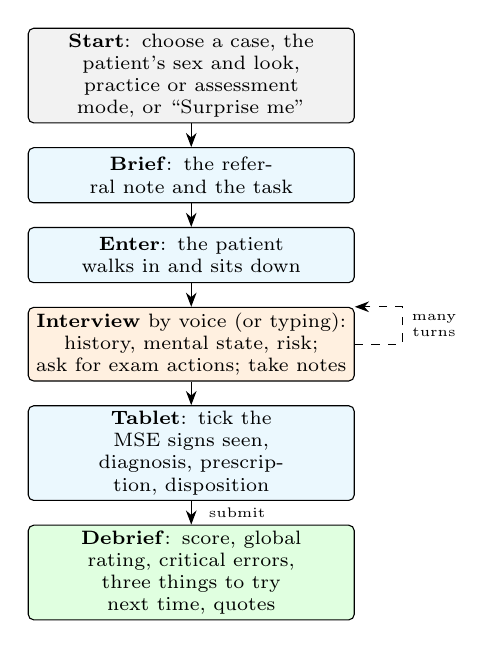
\begin{tikzpicture}[node distance=3mm]
\tikzset{b/.style={box=#1, text width=40mm}}
\node[b=gray!10] (s) {\textbf{Start}: choose a case, the patient's sex and look,\\practice or assessment mode, or ``Surprise me''};
\node[b=cyan!8, below=of s] (b) {\textbf{Brief}: the referral note and the task};
\node[b=cyan!8, below=of b] (e) {\textbf{Enter}: the patient walks in and sits down};
\node[b=orange!12, below=of e] (a) {\textbf{Interview} by voice (or typing):\\history, mental state, risk;\\ask for exam actions; take notes};
\node[b=cyan!8, below=of a] (t) {\textbf{Tablet}: tick the MSE signs seen,\\diagnosis, prescription, disposition};
\node[b=green!12, below=of t] (d) {\textbf{Debrief}: score, global rating, critical errors,\\three things to try next time, quotes};
\draw[->] (s) -- (b); \draw[->] (b) -- (e); \draw[->] (e) -- (a); \draw[->] (a) -- (t); \draw[->] (t) -- node[lab, right, xshift=1mm]{submit} (d);
\draw[->, dashed] (a.east) -- ++(6mm,0) |- node[lab, right, pos=0.25]{many\\turns} (a.north east);
\end{tikzpicture}
\caption{A student's path through one station. In assessment mode the station also ends when time runs out.}
\label{fig:journey}
\end{figure}

Fig.~\ref{fig:journey} shows a student's path. On the start screen the student picks a case, the patient's sex and body, and a mode. \emph{Practice}
mode allows any conversation style; \emph{assessment} mode keeps the authored style for everyone and stops at the time limit (15 minutes for the
depression case). ``Surprise me'' picks a random patient seed: the same clinical case, but different everyday details and a different conversation
style. After a short brief, the patient walks in and sits down. The student talks out loud; the patient answers with a designed voice, and its face,
gaze and posture change with its feelings. The student can ask for physical examination actions (``hold out your hands'', ``roll up your sleeves'',
``follow my finger'', ``stand up and walk''), and can type instead of speak. On a tablet the student records the mental-status signs they saw, a
diagnosis, a prescription and a plan. Then they submit and get a debrief.

\begin{table}[t]
\caption{The four draft stations}
\label{tab:stations}
\centering
\scriptsize
\begin{tabularx}{\columnwidth}{@{}lY@{}}
\toprule
Station & What the student must do\\
\midrule
Moderate depression & Assess a 24-year-old software tester with two months of low mood, early waking, weight loss and a passive wish not to wake up; find no
plan and no means; recognise depression and plan care.\\
``I want to go home'' & On a ward, the same patient asks to leave; explore reasons, explain rights honestly under the Mental Healthcare Act
\cite{mhca2017}, assess capacity and current risk, offer choices.\\
``I'm not taking those tablets'' & A young, guarded patient refuses medicine; uncover side effects, beliefs about the tablets and voices; assess
understanding and risk.\\
Alcohol withdrawal & A sales manager with shaking hands, about 12 hours after his last drink, with a past withdrawal fit; find the real amount, morning
drinking and the fit; plan supervised withdrawal \cite{nice2010cg100}.\\
\bottomrule
\end{tabularx}
\end{table}

\section{System}
\subsection{Overview}

\begin{figure}[t]
\centering
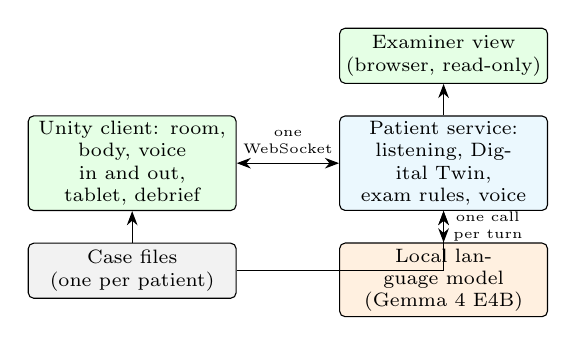
\begin{tikzpicture}[node distance=4mm]
\tikzset{b/.style={box=#1, text width=25mm}}
\node[b=green!10] (u) {Unity client: room,\\body, voice in and out,\\tablet, debrief};
\node[b=cyan!8, right=13mm of u] (s) {Patient service:\\listening, Digital Twin,\\exam rules, voice};
\node[b=orange!12, below=of s] (l) {Local language model\\(Gemma 4 E4B)};
\node[b=gray!10, below=of u] (c) {Case files\\(one per patient)};
\node[b=green!10, above=of s] (v) {Examiner view\\(browser, read-only)};
\draw[<->] (u) -- node[lab, above]{one\\WebSocket} (s); \draw[<->] (s) -- node[lab, right]{one call\\per turn} (l);
\draw[->] (c) -- (u); \draw[->] (c) -| (s); \draw[->] (s) -- (v);
\end{tikzpicture}
\caption{Rapport's parts, all on one laptop.}
\label{fig:overview}
\end{figure}

Three programs run on one laptop (Fig.~\ref{fig:overview}): a Unity~6 client (room, patient, interface, microphone, lip sync); a Python patient service
(listening and turn-end detection, speech recognition, the Digital Twin, rules for exam requests, and speech with Qwen3-TTS VoiceDesign and a KittenTTS
fallback); and llama.cpp \cite{llamacpp} running Gemma 4 E4B, a 4-billion-parameter model compressed to 4 bits, made to answer in valid JSON. No audio or
text leaves the laptop; only the read-only examiner view can be opened from another device on the same network.

\subsection{Case files}
Each patient is a file that lists: who they are and their body and voice for each sex; their memories, each with a trust level, example questions and
topics; a mental-status profile; a starting state; visible signs (tremor, sweating, slumping); examination findings; rating-scale scores (PHQ-9 and
GAD-7, or AUDIT and CIWA-Ar); clinical words the patient must never use; a formulation; and a hidden answer key (diagnosis, differentials, required and
critical questions, safe and unsafe prescriptions, disposition). Everyday details (a hobby, a sibling's name, a home town) and the conversation style can
vary with a seed, while the answer key stays fixed. Ward stations add events whose timing code decides.

\subsection{The Digital Twin}
Each turn the Twin:
\begin{enumerate}
\item finds the memories the doctor's words touch, by keywords and by meaning, then applies the trust locks, so a locked memory gives only a sign of
discomfort;
\item reads what the doctor just did (empathy, judgement, jargon, a risk question and others), changes trust, updates how guarded the patient is by fixed
rules, and makes a short list of allowed behaviours;
\item makes one call to the language model, which may only choose among the allowed behaviours, and writes the behaviour and emotion before the words;
\item checks every sentence before it is spoken (wrong numbers and names corrected; the death wish never spoken when locked or unasked, and never flatly
denied when unlocked and asked kindly);
\item updates trust, mood (pleasure, arousal, dominance \cite{mehrabian1996pad}) and a memory of the conversation: what was asked and said, promises and
hurts.
\end{enumerate}
The companion paper on the Twin gives the exact rules and their validation.

\subsection{Speed}
Five changes cut the median wait from 3.0\,s to 1.6\,s with the earlier voice: the deliberate pause for psychomotor slowing now overlaps the computing
time; a template change stopped stray ``thinking'' that blocked the reply format; reply fields were bounded; the next turn's prompt is prepared while
the doctor is still talking; and the silence needed to end a turn was shortened. A playback hold keeps the new, more expressive voice smooth when the
language model and the voice share the graphics chip.

\subsection{Examiner view}
A web page shows the Twin live: gauges for trust, distress, agitation and engagement, a mood plot, memories unlocking as trust rises, the formulation, and a
one-line reason for each reply written by code. An examiner can watch it on a second laptop.

\subsection{Body and examination}
Requests such as ``hold out your hands'' are recognised by rules, allowed or refused by trust and agitation, queued, held until ``relax'', and acted out
with inverse kinematics: palms turn, sleeves roll up, held hands show a fine tremor (about 10\,Hz) or a coarse withdrawal tremor (5--6\,Hz), and sweat
shows as a sheen. Between words the patient blinks, breathes, shifts in the chair and looks at or away from the doctor depending on trust; when the Twin
decides an emotion, the body leans in (anger), fidgets (anxiety), slumps and looks down (sadness) or smiles (happiness) (Fig.~\ref{fig:bodies}).

\begin{figure}[t]
\centering
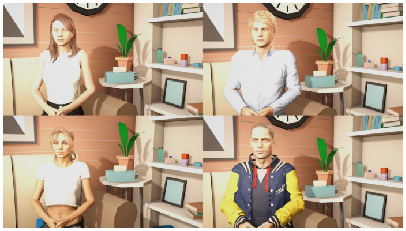
\includegraphics[width=\columnwidth]{fig_bodies.pdf}
\caption{The four patient bodies from the doctor's seat.}
\label{fig:bodies}
\end{figure}

\subsection{Scoring and debrief}

\begin{figure}[t]
\centering
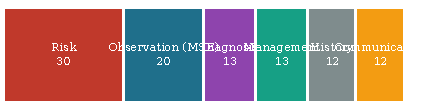
\includegraphics[width=\columnwidth]{fig_debrief_weights.pdf}
\caption{How the 100 debrief points are divided, risk first.}
\label{fig:weights}
\end{figure}

The debrief is scored by code from what happened in the session, with risk weighted most (Fig.~\ref{fig:weights}):
\begin{itemize}
\item \textbf{Risk (30).} Each risk item, plus the case's critical items (for example, past withdrawal fits), scores full marks when asked and answered,
60\% when asked before the patient trusted the student enough to answer, and zero with a critical error when not asked. No risk ``category'' is printed,
following NICE guidance \cite{nice2022ng225}.
\item \textbf{Observation (20).} The expected mental-status signs are the ones the patient actually showed for at least 5\,s; ticking signs that were not
there costs marks.
\item \textbf{History, diagnosis and management (12, 13, 13).} Questions covered, the diagnosis and differentials, and a safe prescription and plan.
\item \textbf{Communication (12).} Six items from the Master Interview Rating Scale and the Calgary--Cambridge guides \cite{simmenroth2014calgary}
(introduction, confidentiality, open questions, empathy, summarising, checking understanding), with deductions for judgmental lines, real interruptions,
jargon and stacked questions.
\end{itemize}
The debrief ends with a global rating, the three most important things to try next time with words to use, and comments that quote the student's own
lines. Optional AI examiner notes rate eight verbal items; every quote is checked against the transcript, and the notes never change the score.

\section{Evaluation Design}
\begin{table}[t]
\caption{Research questions and their status}
\label{tab:rq}
\centering
\scriptsize
\begin{tabularx}{\columnwidth}{@{}lYY@{}}
\toprule
RQ & Question & How measured (status)\\
\midrule
RQ1 & Is it fast enough to talk to? & Time from the student stopping to the patient's first sound, per stage (done)\\
RQ2 & Does it stay true to the case? & Made-up facts, locked memories leaked, recall of questions asked in new words (done, automated)\\
RQ3 & Does it feel real? & Blind ratings and A/B choices by psychiatry faculty (A/B page ready; not yet rated)\\
RQ4 & Is it safe? & Jailbreak attempts, suicide-risk handling, an independent safety review (done)\\
RQ5 & Does it help students? & Interview rubric, MSE and diagnosis accuracy, usability (waiting for ethics approval)\\
\bottomrule
\end{tabularx}
\end{table}
Table~\ref{tab:rq} lists the research questions. Studies with people need ethics approval first. Automated testing uses 14 scripted conversations
never used for tuning (12 for depression, 2 for alcohol withdrawal), each run with three random seeds and marked by an AI model different from the
patient's, with every flag checked by hand; a blind set of 512 questions for memory recall; and an independent safety review by an AI agent with no
prior context.

\section{Results}

\begin{table}[t]
\caption{How Rapport developed (2026)}
\label{tab:history}
\centering
\scriptsize
\begin{tabularx}{\columnwidth}{@{}lY@{}}
\toprule
Version (date) & What changed, with key numbers\\
\midrule
Twin 0.1 (20 Oct) & Live Digital Twin; median wait 3.0\,s $\to$ 1.6\,s\\
v0.2 (21 Oct) & Exam rules (385 sentences, 100\%); expressive voice; learning loop (one learned version rejected for a safety flag)\\
v0.2.1 (22 Oct) & New demo interview; three recall bugs found and fixed\\
Personalities (22--31 Oct) & Seeded patients, six styles, ward events, alcohol case, scoring overhaul, life stories\\
v0.3 (13--14 Nov) & Code decides before the model; meaning-based recall; memory of the conversation; checks before speech; body language;
conversation-distance camera\\
\bottomrule
\end{tabularx}
\end{table}

Table~\ref{tab:history} shows how the system developed.

\textbf{RQ1, speed.} The median wait fell from 3.0\,s to 1.6\,s through the speed changes above (earlier voice, 26 turns). With the expressive voice and
the current Twin it is 1.82\,s (90th percentile 2.96\,s, 37 turns), against 1.54\,s for the previous Twin (80 turns). The 1.2\,s target is not met. When
the student talks over the patient, the patient stops within 47--63\,ms.

\begin{table}[t]
\caption{Held-out results, previous Twin (v0) and current Twin (v2), three seeds}
\label{tab:res}
\centering
\footnotesize
\begin{tabular}{@{}lcc@{}}
\toprule
& v0 & v2\\
\midrule
Accuracy (composite), depression / alcohol & 0.953 / 0.878 & 0.947 / 0.875\\
Share of turns in top two behaviours & 0.86 / 0.81 & 0.72 / 0.63\\
Resistance fits the situation & 0.92 / 0.67 & 0.94 / 0.70\\
Jailbreak / portrayal failures & 1 / 0 & 0 / 0\\
Suicidal thoughts disclosed when unlocked, asked kindly & every run & every run\\
Risk questions in new words found (test set) & 35.1\% & 72.7\%\\
\bottomrule
\end{tabular}
\end{table}

\textbf{RQ2 and RQ4, staying true and safe.} Table~\ref{tab:res} compares the two Twins. The current Twin passed every safety check with the same accuracy
and much more varied behaviour. Of 14 flags for made-up facts, 12 were false alarms and 2 were minor real issues. Earlier automated results still stand:
the previous Twin's tests showed 100\% valid output and no made-up facts after review (18 of 18 flags were false alarms); one character break (``Yes, I
know'' to ``This is just a simulation, right?'') was found and fixed; a learned version was rejected because it denied suicidal thoughts at high trust,
which was traced to a missing keyword; across four conversation styles the death wish was disclosed in 8 of 8 kind requests with no locked memory
leaked; and in the ward station a coercive doctor drove trust from 25 to 0 while a calming one raised it to 70. An independent safety review of the
current Twin found ten defects (for example, the raw text of a reply whose every sentence had been dropped still reached the client); all were fixed
and tested before the results above.

\textbf{RQ3 and RQ5.} There are no faculty ratings or student data yet. A blind A/B page with ten pairs of held-out replies is ready.

\section{Discussion, Limitations and Ethics}
Moving the patient's decisions into code made its behaviour something an examiner can inspect and a reviewer can test, and the body now shows the same
decision as the voice.

\textbf{Limitations.}
\begin{itemize}
\item Only four draft stations; psychosis, mania and anxiety are not covered yet.
\item All clinical content, trust levels and debrief cut-offs are drafts that psychiatrists must still review.
\item The Twin is inspired by brain science but is not a model of the brain.
\item AI judges are biased, and their flags were checked by the developer, not by faculty.
\item The exam rules' accuracy is optimistic, because one person wrote both the rules and the tests.
\item Recall of risk questions in new words (72.7\%) is below what a safety gate needs, and an upset patient does not yet stay upset for long.
\item Everything was tested on one high-end laptop; the student's own body language is not assessed.
\end{itemize}

\textbf{Ethics.} No real patient data is stored. A student's words never become patient facts, and student sessions are used for learning only with
consent. Suicide-related content comes with a content note and a debrief with teaching points. Voices are designed from written descriptions, not copied
from real people. Demonstrations that use pre-scripted replies must say so.

\begin{table}[t]
\caption{Next steps}
\label{tab:next}
\centering
\scriptsize
\begin{tabularx}{\columnwidth}{@{}YY@{}}
\toprule
Step & Why\\
\midrule
Faculty review of all four cases and the flagged replies & Clinical truth and judge accuracy\\
Faculty blind A/B ratings & Answer RQ3: does it feel real?\\
Ethics approval and a student pilot (n $\approx$ 20--30) & Answer RQ5: does it help?\\
Hand-checked labels and a fine-tuned recall model & Reach 95\% recall on risk questions\\
A psychosis or anxiety case & Broader coverage\\
Lip sync and skin, eye and hair shading & More lifelike face up close\\
\bottomrule
\end{tabularx}
\end{table}

\section{Conclusion}
Rapport shows that a spoken, embodied psychiatric standardised patient can run privately on one laptop, with a patient mind whose decisions an examiner
can see and a reviewer can test. Whether it is real enough, and useful enough, to teach with is the next question (Table~\ref{tab:next}), and it needs
psychiatrists and students to answer it.

\bibliographystyle{IEEEtran}
\bibliography{../shared/refs}

\end{document}
